\documentclass[10pt]{book}
\usepackage[sectionbib]{natbib}
\usepackage{array,epsfig,fancyhdr,rotating}
\usepackage[driverfallback=dvipdfm]{hyperref}
%%%%%%%%%%%%%%%%%%%%%%%%%%%%%%%%%%%%%%%%%%%%%%%%%%%%%%%%%%%%%%%%%%%%%%%%%%%%%%%%%%%%%%%%%%%%%%%%%%%%%%%%%%%%%%%%%%%%%%%%%%%%

\textwidth=31.9pc
\textheight=46.5pc
\oddsidemargin=1pc
\evensidemargin=1pc
\headsep=15pt
%\headheight=.2cm
\topmargin=.6cm
\parindent=1.7pc
\parskip=0pt

\usepackage{amsmath}
\usepackage{amssymb}
\usepackage{amsfonts}
\usepackage{multirow}
\usepackage{amsthm}
\usepackage[export]{adjustbox}

\setcounter{page}{1}
\newtheorem{theorem}{Theorem}
\newtheorem{lemma}{Lemma}
\newtheorem{corollary}{Corollary}
\newtheorem{proposition}{Proposition}
\theoremstyle{definition}
\newtheorem{definition}{Definition}
%\newtheorem{proof}{Proof}
\newtheorem{example}{Example}
\newtheorem{remark}{Remark}
\pagestyle{fancy}

% List labels
\usepackage{scrextend}
\addtokomafont{labelinglabel}{\sffamily}

%%%%%%%%%%%%%%%%%%%%%%%%%%%%%%%%%%%%%%%%%%%%%%%%%%%%%%%%%%%%%%%%%%%%%%%%%%%%%%%%%%%%%%%%%%%%%%%%%%%%%%%%%%%%%%%%%%%%%%%%%%%%
\pagestyle{fancy}
\def\n{\noindent}
\lhead[\fancyplain{} \leftmark]{}
\chead[]{}
\rhead[]{\fancyplain{}\rightmark}
\cfoot{}
\renewcommand{\headrulewidth}{0pt}

%%%%%%%%%%%%%%%%%%%%%%%%%%%%%%%%%%%%%%%%%%%%%%%%%%%%%%%%%%%%%%%%%%%%%%%%%%%%%%%%%%%%%%%%%%%%%%%%%%%%%%%%%%%%%%%%%%%%%%%%%%%%
%%%%%%%%%%%%%%%%%%%%%%%%%%%%%%%%%%%%%%%%%%%%%%%%%%%%%%%%%%%%%%%%%%%%%%%%%%%%%%%%%%%%%%%%%%%%%%%%%%%%%%%%%%%%%%%%%%%%%%%%%%%%

\begin{document}

%%%%%%%%%%%%%%%%%%%%%%%%%%%%%%%%%%%%%%%%%%%%%%%%%%%%%%%%%%%%%%%%%%%%%%%%%%%%%%%%%%%%%%%%%%%%%%%%%%%%%%%%%%%%%%%%%%%%%%%%%%%%
%%%%%%%%%%%%%%%%%%%%%%%%%%%%%%%%%%%%%%%%%%%%%%%%%%%%%%%%%%%%%%%%%%%%%%%%%%%%%%%%%%%%%%%%%%%%%%%%%%%%%%%%%%%%%%%%%%%%%%%%%%%%

\renewcommand{\baselinestretch}{2}

\markright{ \hbox{\footnotesize\rm Statistica Sinica
%{\footnotesize\bf 24} (201?), 000-000
}\hfill\\[-13pt]
\hbox{\footnotesize\rm
%\href{http://dx.doi.org/10.5705/ss.20??.???}{doi:http://dx.doi.org/10.5705/ss.20??.???}
}\hfill }

\markboth{\hfill{\footnotesize\rm JASON POULOS AND RAFAEL VALLE} \hfill}
{\hfill {\footnotesize\rm MISSING DATA IMPUTATION FOR NEURAL NETWORKS} \hfill}

\renewcommand{\thefootnote}{}
$\ $\par

%%%%%%%%%%%%%%%%%%%%%%%%%%%%%%%%%%%%%%%%%%%%%%%%%%%%%%%%%%%%%%%%%%%%%%%%%%%%%%%%%%%%%%%%%%%%%%%%%%%%%%%%%%%%%%%%%%%%%%%%%%%%

\fontsize{12}{14pt plus.8pt minus .6pt}\selectfont \vspace{0.8pc}
\centerline{\large\bf MISSING DATA IMPUTATION FOR NEURAL NETWORKS}
%\vspace{2pt} \centerline{\large\bf IF A SECOND LINE IS NEEDED}
\vspace{.4cm} \centerline{Jason Poulos and Rafael Valle} \vspace{.4cm} \centerline{\it
University of California, Berkeley} \vspace{.55cm} \fontsize{9}{11.5pt plus.8pt minus
.6pt}\selectfont

%%%%%%%%%%%%%%%%%%%%%%%%%%%%%%%%%%%%%%%%%%%%%%%%%%%%%%%%%%%%%%%%%%%%%%%%%%%%%%%%%%%%%%%%%%%%%%%%%%%%%%%%%%%%%%%%%%%%%%%%%%%%

\begin{quotation}
\noindent {\it Abstract:}
Researchers analyzing survey data typically choose decision trees or random forests for prediction tasks, largely because missing data and categorical variables are not easy to handle with neural networks. This paper investigates techniques for handling missing categorical data such that it is appropriate to neural network classifiers. We experiment on two benchmark datasets with missing categorical data, comparing a four-layer neural network with decision tree and random forests classifiers trained on differently imputed data and various levels of perturbation. We beat the state-of-the-art test error on both datasets using a random forests classifier, either trained on data imputed with logistic regression or data with one-hot encoding. We conclude from the results that the performance of the classifiers and imputation strategies generally depend on the nature and proportion of missing data. \par

\vspace{9pt}
\noindent {\it Key words and phrases:}
missing data, imputation methods, neural networks, random forests
%Balanced incomplete block design, Hadamard matrix, nearly balanced incomplete block design, orthogonal array.
\par
\end{quotation}\par



\def\thefigure{\arabic{figure}}
\def\thetable{\arabic{table}}

\fontsize{12}{14pt plus.8pt minus .6pt}\selectfont

\setcounter{chapter}{1}
\setcounter{equation}{0} %-1
\noindent {\bf 1. Introduction} 

Missing data is a common problem in survey data in various domains. Random Forests and other decision tree methods are the method of choice for survey data, largely because missing data are not easy to handle with neural networks. We investigate techniques for handling missing categorical data such that it is appropriate to neural network classifiers. We assess the performance of neural network classifiers in comparison with decision tree and random forests classifiers trained on differently imputed data and for various degrees of perturbation.

After briefly reviewing related works in Section 2 we experiment on benchmark datasets and compare our results with the state-of-the-art in Section 3. Finally, we draw conclusions in Section 4.
\par

\lhead[\footnotesize\thepage\fancyplain{}\leftmark]{}\rhead[]{\fancyplain{}\rightmark\footnotesize\thepage}%Put this line in Page 2

\setcounter{chapter}{2}
\setcounter{equation}{0} %-1
\noindent {\bf 2. Related work}

\noindent {\bf 2.1. Neural networks for classification with categorical and continuous features}

Common techniques for handling categorical data in
neural networks include encoding the categorical values into numeric values
or using binary encoding. These techniques, however, have some drawbacks
including unnecessarily increasing model complexity or feature dimensionality
and not preserving the similarity information embedded between categorical
values \citep{hsu2006generalizing}. More elaborate techniques include information theoretic measures
\citep{wang2008categorical}, training separate output units for
each of the allowed combination of values of the categorical independent
variables \citep{brouwer2002feed}, and using distance
hierarchies \citep{hsu2006generalizing}. 

In the case of categorical variables, which by definition have no direct
representation or computation scheme of the distance between its values,
decision trees can be useful because they do not require distance metrics.
However, their training process is slow given a large enough dataset and they
might not be suitable for problems where the decision boundary between classes
described by a second-order polynomial, for example \citep{fayyad1996data}.

\noindent {\bf 2.2. Techniques for handling missing data} \label{section:techniques}
Several techniques for data imputation (i.e., replace missing values with plausible ones) and
direct estimation (i.e., all missing data is analyzed using a maximum likelihood
approach) have been proposed \citep{de2003prevention}. We compare seven different imputation techniques within the following five categories which are commonly found in the previous work on missing data imputation \citep{batista2003analysis}:

\begin{labeling}{MDI}

\item[$k$-nearest-neighbors ($k$-NN)]
Compute the $k$-NN of the observation with missing data and assign the mode of the $k$-neighbors to the missing data.

\item[Classification algorithm]
Train a classification algorithm --- such as logistic regression, random forests or support vector machines (SVMs) --- to classify missing data given existing data. 

%\item[Principal component analysis (PCA)]
%Perform factor analysis (e.g., PCA) on the design matrix, project the design matrix onto the first $N$ eigenvectors and replace the missing values by the values that might be given by the projected design matrix.

\item[Random replacement] 
One observation with missing data is randomly replaced with another non-sampled observation.

\item[Mode replacement]
Replace the missing data with the mode of the corresponding feature vector of the training set.

\item[One-hot] Create a binary variable to indicate whether or not a specific feature is missing.

\end{labeling}

\par

%%%%%%%%%%%%%%%%%%%%%%%%%%%%%%%%%%%%%%%%%%%%%%%%%%%%%%%%%%%%%%%%%%%%%%%%%%%%%%%%%%%%%%%%%%%%%%%%%%%%%%%%%%%%%%%%%%%%%%%%%%%%
%\newpage

\setcounter{chapter}{3}
\setcounter{equation}{0} %-1
\noindent {\bf 3. Experiments} 

\noindent {\bf 3.1. Benchmark data sets}

We experiment on two benchmark datasets from the UCI Machine Learning Repository: the Adult dataset and Congressional Voting Records (CVRs) dataset \citep{Lichman2013}. The Adult dataset contains $N=48,842$ observations and 14 features (6 continuous and 8 categorical). Missing values in this dataset are unknown survey responses. The prediction task is to determine whether a person makes over \$50,000 a year. The CVRs dataset contains $N=435$ observations, each the voting record of a member of the $98^{th}$ U.S. House of Representatives for 16 key roll call votes identified by the Congressional Quarterly Almanac. Thus, the dataset contains 16 categorical features with three possible values: ``yea'', ``nay'', and missing. Missing values in this dataset are not simply unknown, but represents values other up-or-down votes, such as voted present, voted present to avoid conflict of interest, and did not vote or otherwise make a position known. The prediction task is to classify party affiliation (Republican or Democrat). 

We randomly split each dataset $2/3$ for training and $1/3$ for testing. The state--of--the--art for the Adult dataset is a Naive Bayes classifier that achieves a 14.05\% generalization error after removing samples with missing values \citep{kohavi1996}. The CVRs dataset donor claims to achieve a 90-95\% accuracy using an incremental decision tree algorithm called STAGGER, although it is not known what train-test split is used or how missing values are handled \citep{schlimmer1987,schlimmer1986}.

\par
\noindent {\bf 3.2. Patterns of missing values}

Uncovering patterns of missing values in the dataset will help select strategies for imputing missing values. Figure \ref{fig:proportion-missing-adult} analyzes patterns of missing data in the Adult dataset, in which 7.4\% of the observations contain missing values. Missing values occur in three of the categorical features: \textit{Work class}, \textit{Occupation}, and \textit{Native country}. Since these the former two features are related, it is unlikely that these values are missing completely at random (MCAR); it is more likely, and much less desirable that the values are not missing at random (MNAR). The histogram (left) in Figure \ref{fig:proportion-missing-votes} shows \textit{Work class} and \textit{Occupation} each have about 5.6\% of missing values, and \textit{Native country} has about 1.7\% missing values. The aggregation plot (right) shows 5.5\% of samples are missing values for both \textit{Work class} and \textit{Occupation}. Less than 2\% of samples are missing just \textit{Native country} and less than 1\% are missing all three features.

\begin{figure}[h!]
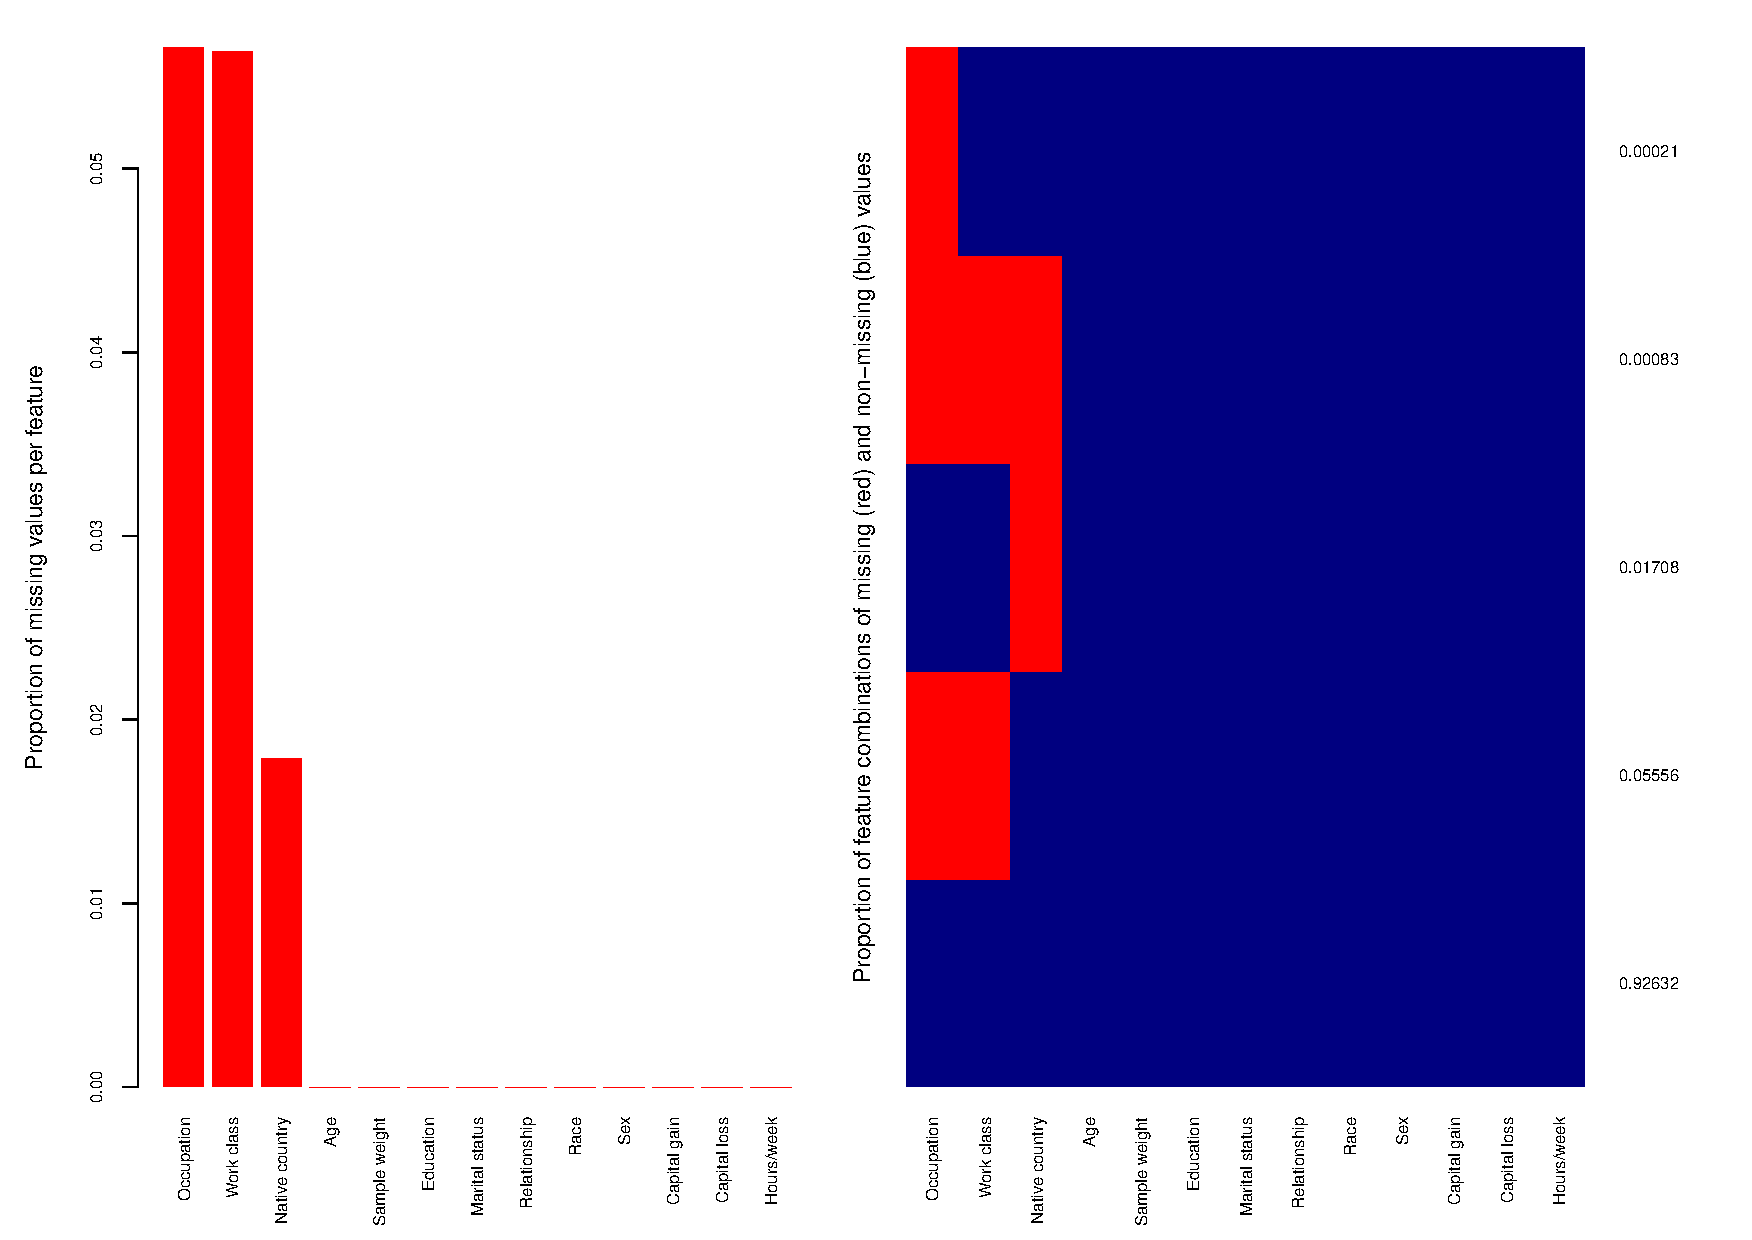
\includegraphics [scale=0.45]{figure/proportion-missing-adult.pdf}\par
\caption{\footnotesize Histogram of proportion of missing values in each feature (Left) of Adult training set and aggregation plot of all existing combinations of missing and non-missing values in the samples (Right).}
 \label{fig:proportion-missing-adult}
\end{figure}

Figure \ref{fig:proportion-missing-votes} shows that 46\% of the CVRs data contains missing values and all features contain missing data. About a quarter of missing data is in \texttt{South Africa}, which was a controversial amendment to amend the Export Administration Act to bar U.S. exports to South Africa's apartheid regime. Twelve percent of missing data is in the feature \texttt{Water}, which is a water projects authorizations bill, and 7\% of missing data rests in the feature \texttt{Exports}, which is a tariff bill. 

\begin{figure}[h!]
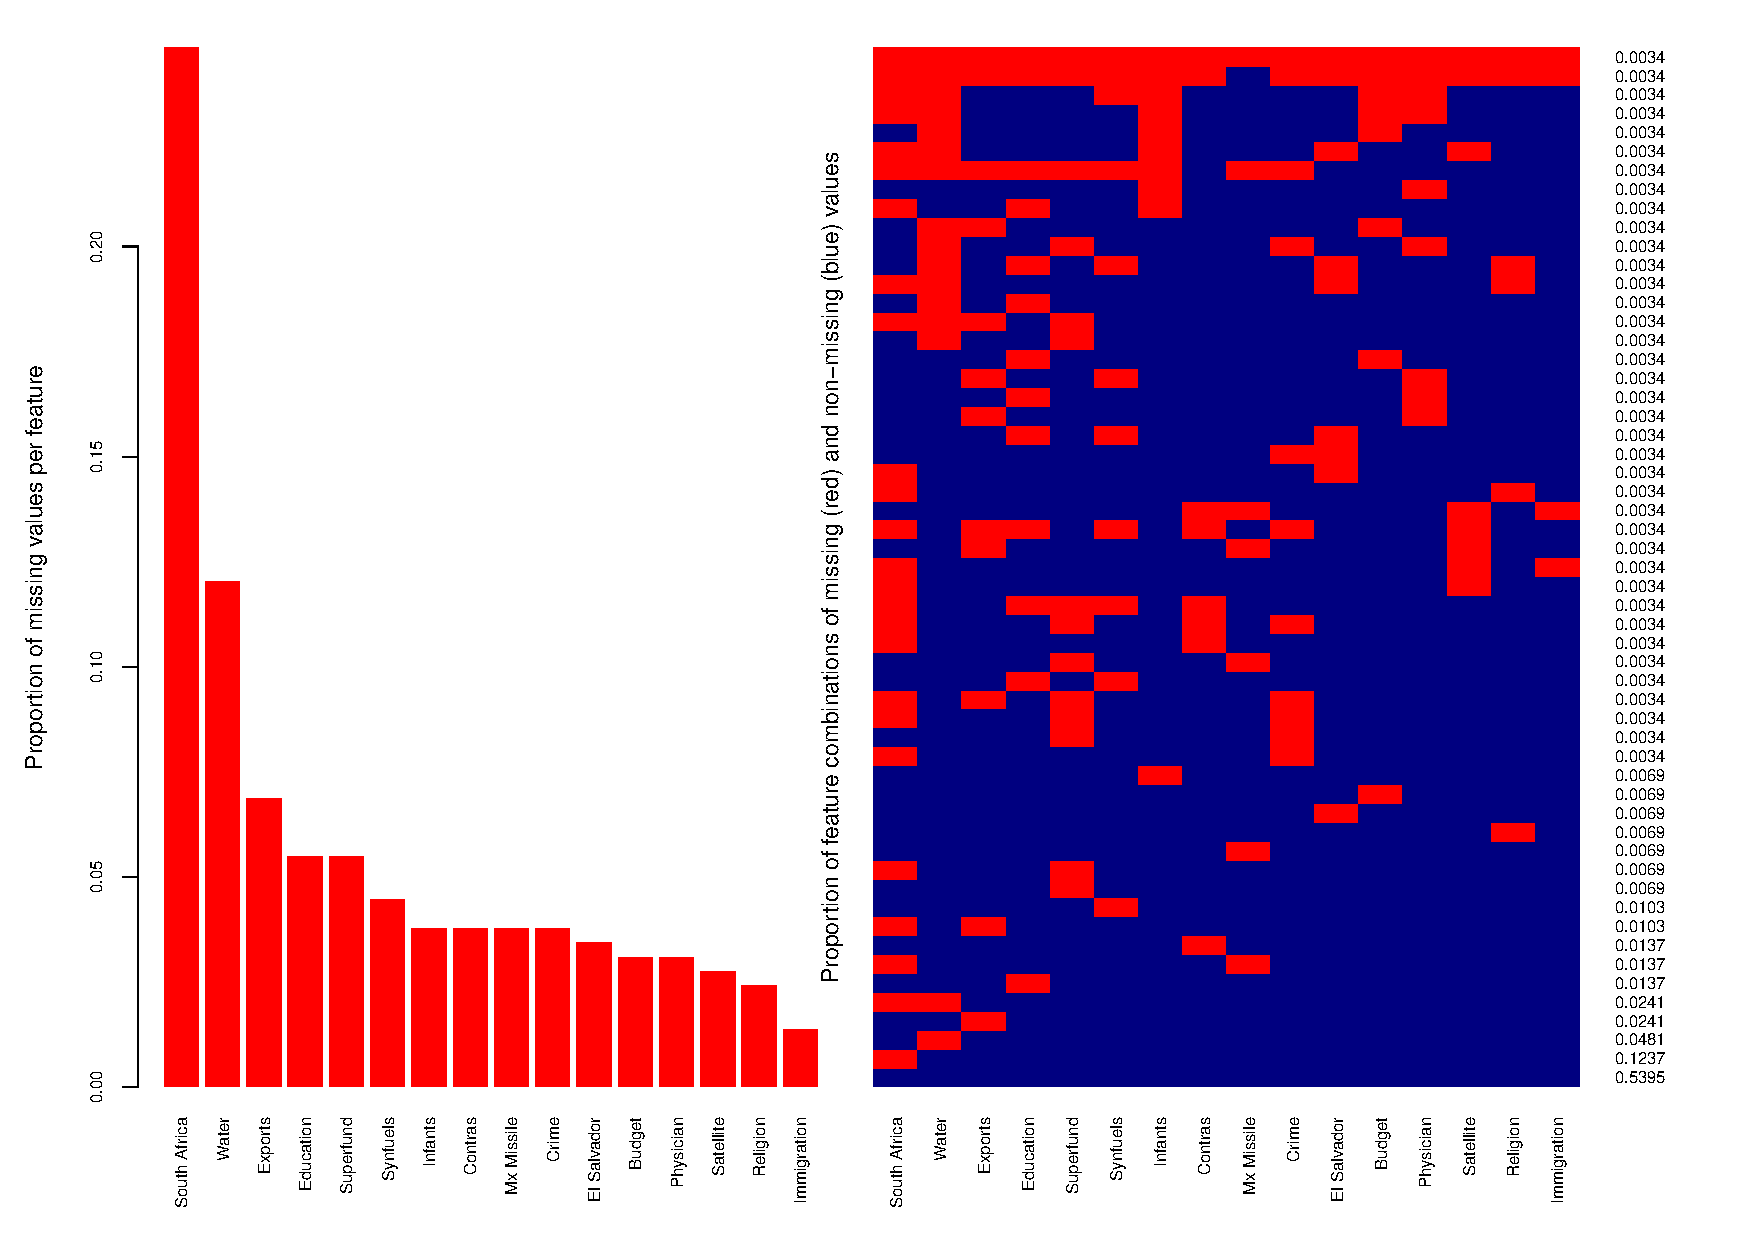
\includegraphics [scale=0.45]{figure/proportion-missing-votes.pdf}\par
\caption{\footnotesize Histogram of proportion of missing values in each feature (Left) of CVRs training set and aggregation plot of all existing combinations of missing and non-missing values in the samples (Right).}
 \label{fig:proportion-missing-votes}
\end{figure}

\par
\noindent {\bf 3.3. Preprocessing}

The first step in preprocessing the training data is artificially increasing the number of missing values in order to study the effect of larger amounts of missing data. We accomplish this by perturbing the categorical training features by substituting nonmissing values with missing values so that each feature has a minimum missing data ratio, from 0-40\%. For example if there 10 categorical features and 10 observations, a missing data ratio of 0.1 will perturb 10 values. Second, we implement one-hot encoding (-1,1) for the categorical variables. Third, we implement the imputation technique. Lastly, we standardize continuous features by subtracting the mean and dividing by the standard deviation of the feature. We preprocess the test data in the same manner, with the exception that there is no perturbation of test features.\footnote{When imputing the missing data with mode replacement, we use the training set mode. We also use the training set mean and standard deviation to standardize test set features.}

\par
\noindent {\bf 3.4. Model training and hyperparameter selection}

We train a four-layer neural network, with each of the two hidden layers having 1024 nodes. We use the adaptive learning rate method Adadelta \citep{zeiler2012} for the update rule. We explore the following hyperparameter space via Bayesian optimization \citep{snoek2012}:

\begin{itemize}
\item Momentum schedule [0 to 1]
\item Dropout regularization [No, Yes]
\item Learning rate: [0.000001 to 0.01].
\end{itemize}

The goal of Bayesian optimization is to choose a point in the hyperparameter space that appropriately balances information gain and exploitation. Figure \ref{fig:params} shows the exploration of hyperparameter space during Bayesian optimization for both Adult and CVRs datasets. Each circle represents a candidate neural network classifier trained on a differently imputed and perturbed dataset. More circles appear in the plot for CVRs simply due to the fact that the training set is smaller. We see that most of the candidate models use dropout and have an initial learning rate close to the maximum of 0.01. The plurality of candidate models appear to either have momentum (1) or not (0). The candidate model with the lowest training error is selected for predicting on the test set. 

\begin{figure}[h!]
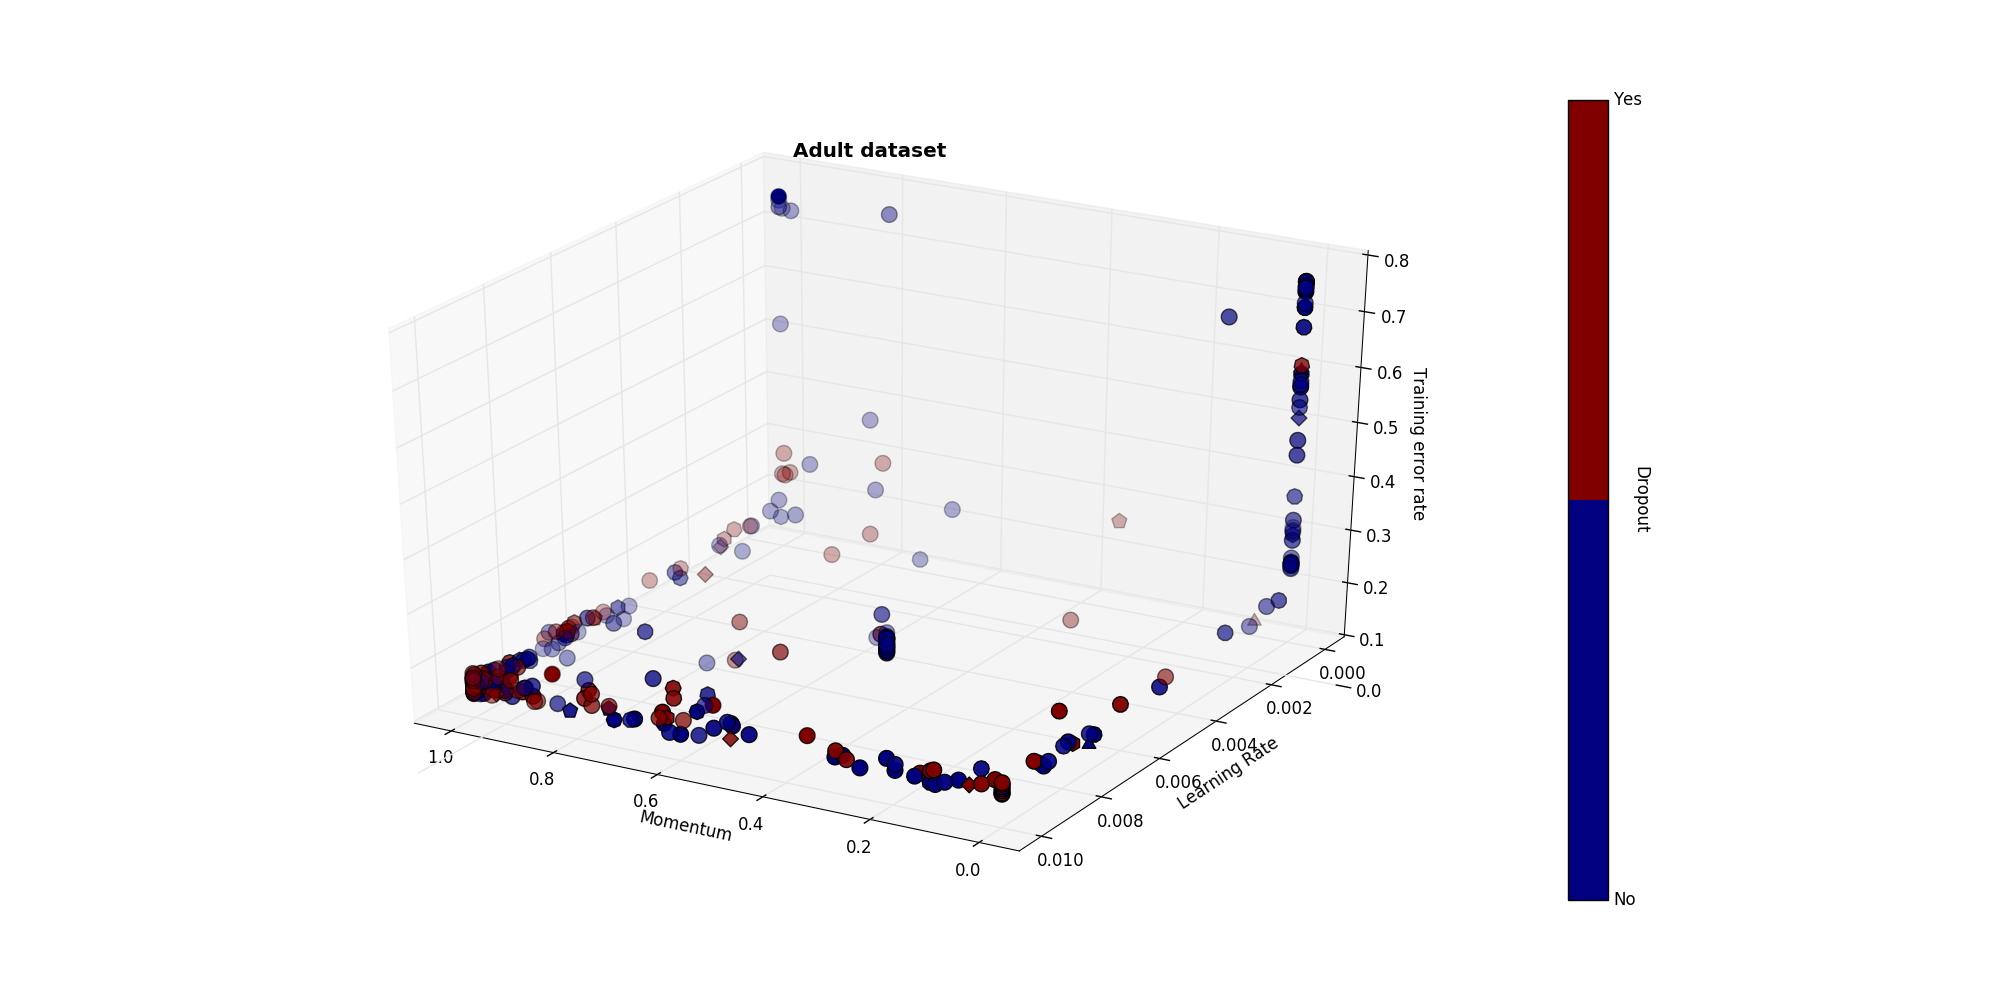
\includegraphics [scale=0.45, center]{../images/params3d_adult.png}\par
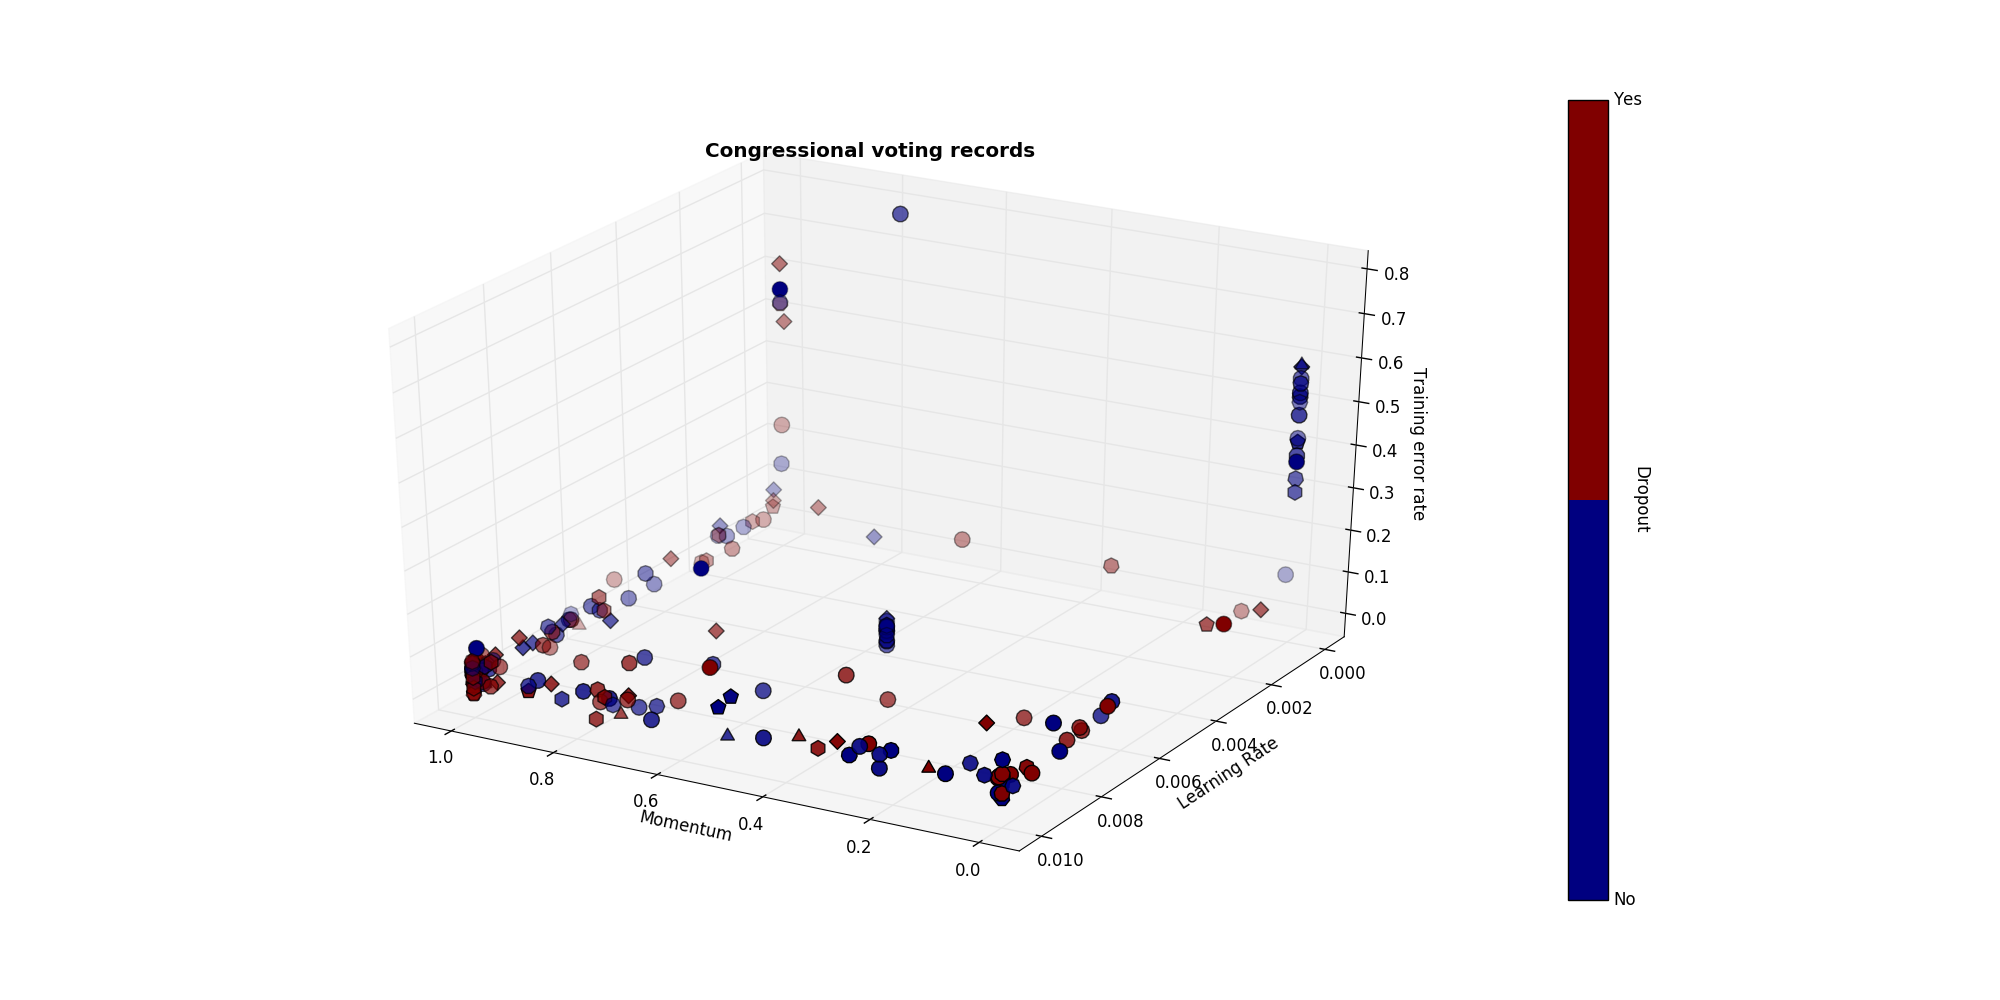
\includegraphics [scale=0.45, center]{../images/params3d_votes.png}\par
\caption{\footnotesize Exploration of hyperparameter space during Bayesian optimization.}
   \label{fig:params}
\end{figure}

\par
\noindent {\bf 3.5. Model assessment}

We assess the performance of the neural network classifier in terms of test set error rate in comparison with decision tree and random forests classifiers on differently imputed data and for various degrees of perturbation.  We use one-hot encoding to represent missing data when no imputation method is used. The results on the Adult dataset and CVRs dataset are plotted in Figures \ref{fig:test-error-adult} and \ref{fig:test-error-votes}, respectively. For the Adult dataset, the random forests classifier trained on data imputed with logistic regression yields the lowest generalization error (13.85\% error), beating the state-of-the-art by 0.2\%. In comparison, random forests trained on data with no missing data imputation matches the state-of-the-art (14.05\%) and neural network trained on data imputed by random replacement performs considerably worse (14.37\%). For the CVRs dataset, random forests trained on one-hot encoded data with up to 20\% of the data perturbed beats the state-of-the-art by over 2\% (2.77\%). Neural networks trained on PCA-imputed data or no imputation also beat the state-of-the-art, with error rates of 3.47\% and 4.16\%, respectively. 

Overall, the performance of the classifiers and imputation strategies depend on the dataset and amount of missing data. For the Adult dataset, random forests classifiers trained on data imputed with other classifiers (i.e., logistic regression, random forests, and SVMs) outperform other classifiers and imputation methods across different ratios of perturbed data. All classifiers trained on one-hot encoded data perform very poorly when the Adult dataset is perturbed. This is likely due to the fact that in the original, non-perturbed Adult dataset, missing values are concentrated in three features which may not be consequential for the prediction task. Perturbation exposes features that are more consequential to the prediction task to missing data. 

Each of the three classifiers trained on one-hot encoded data perform well on the CVRs dataset. In this dataset, missing values represent potentially valuable information for the prediction task and can be more useful for the classifier than the imputed value for certain features. This is why it is not implausible that a classifier trained on perturbed, one-hot encoded data can have lower generalization error than a classifier trained on non-perturbed, one-hot encoded data. 

\begin{figure}[h!]
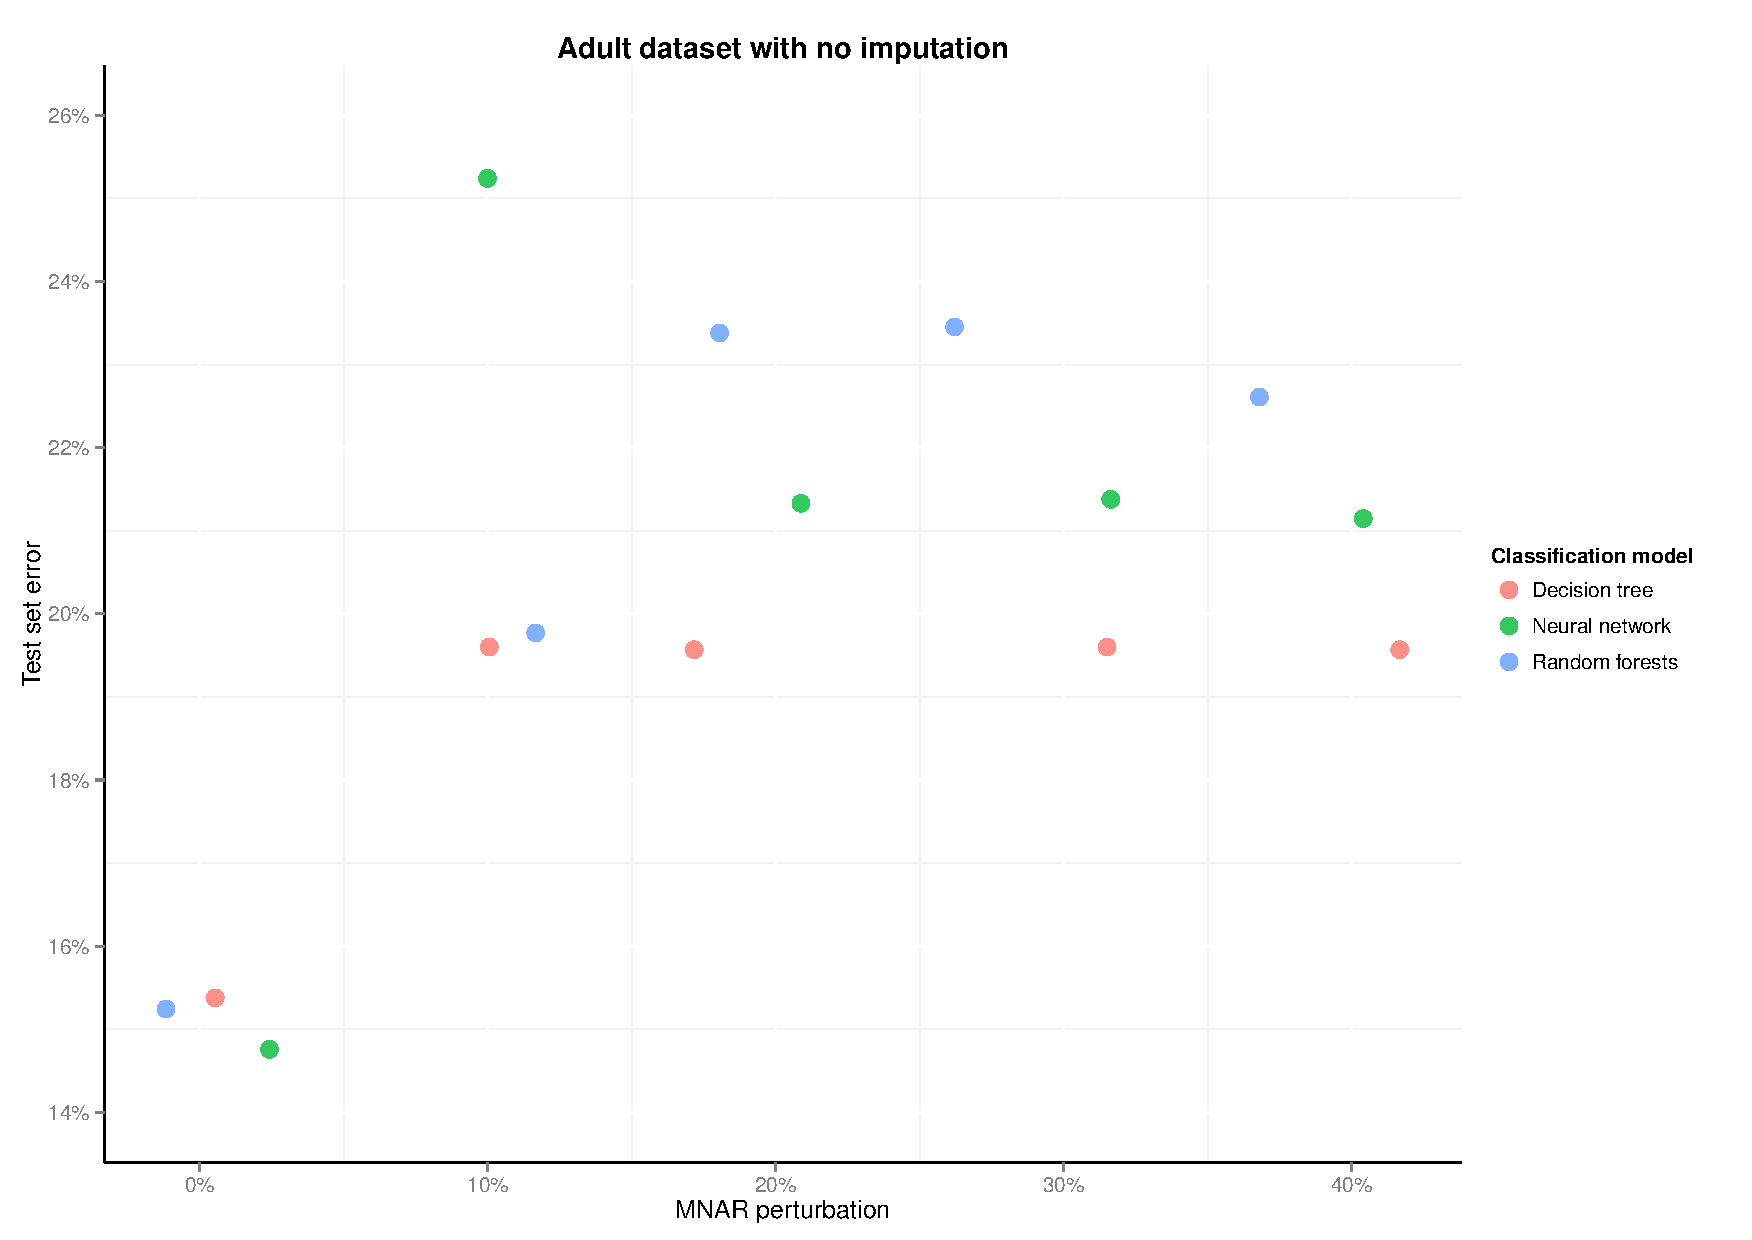
\includegraphics [scale=0.45]{figure/test-errors-adult-no-imp.pdf}\par
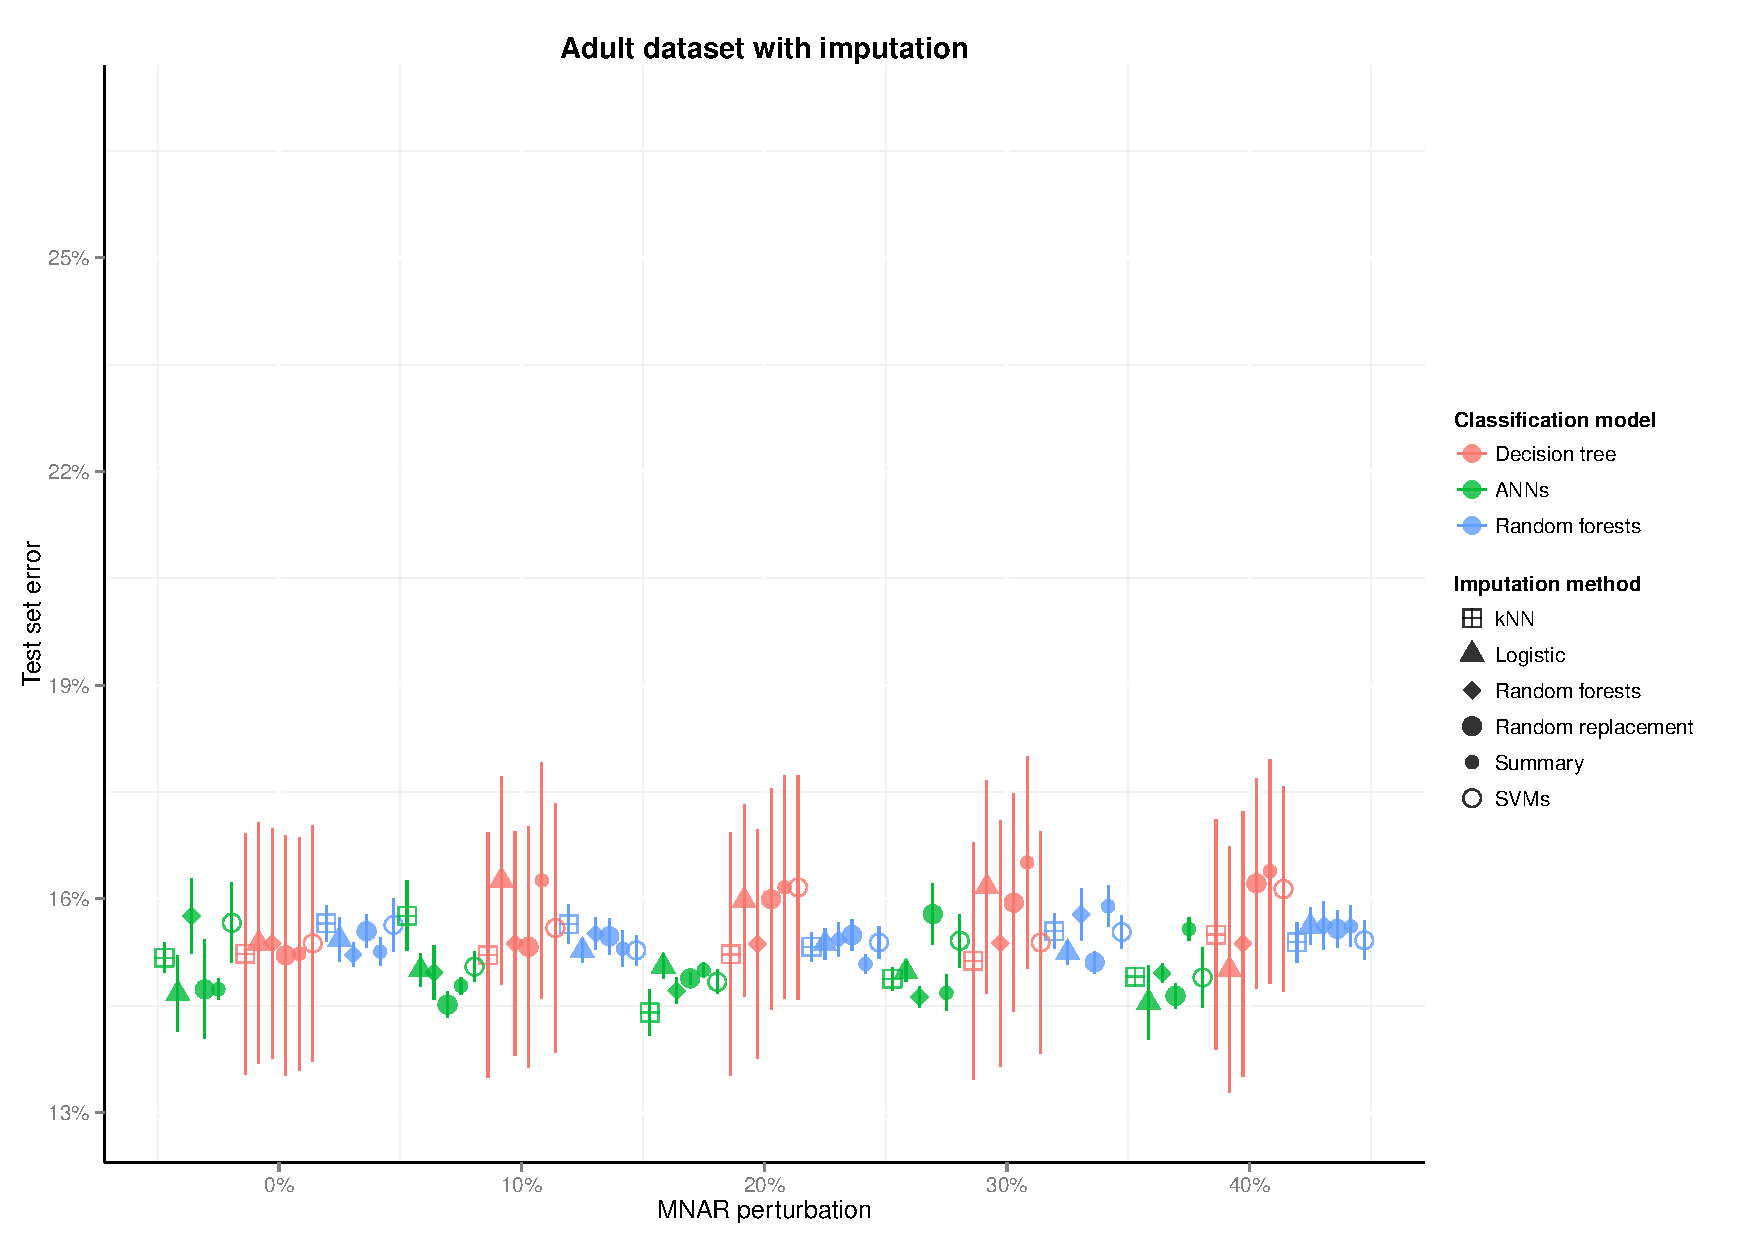
\includegraphics [scale=0.45]{figure/test-errors-adult-imp.pdf}\par
   \caption{\footnotesize Error rates on the Adult test set with (bottom) and without (top) missing data imputation, for various levels of perturbed training features (x-axis). One-hot encoding is used to represent missing data in the absence of imputation. The decision tree and random forests classifiers are trained with maximum depths of 8 and 16, respectively.}
   \label{fig:test-error-adult}
\end{figure}

\begin{figure}[h!]
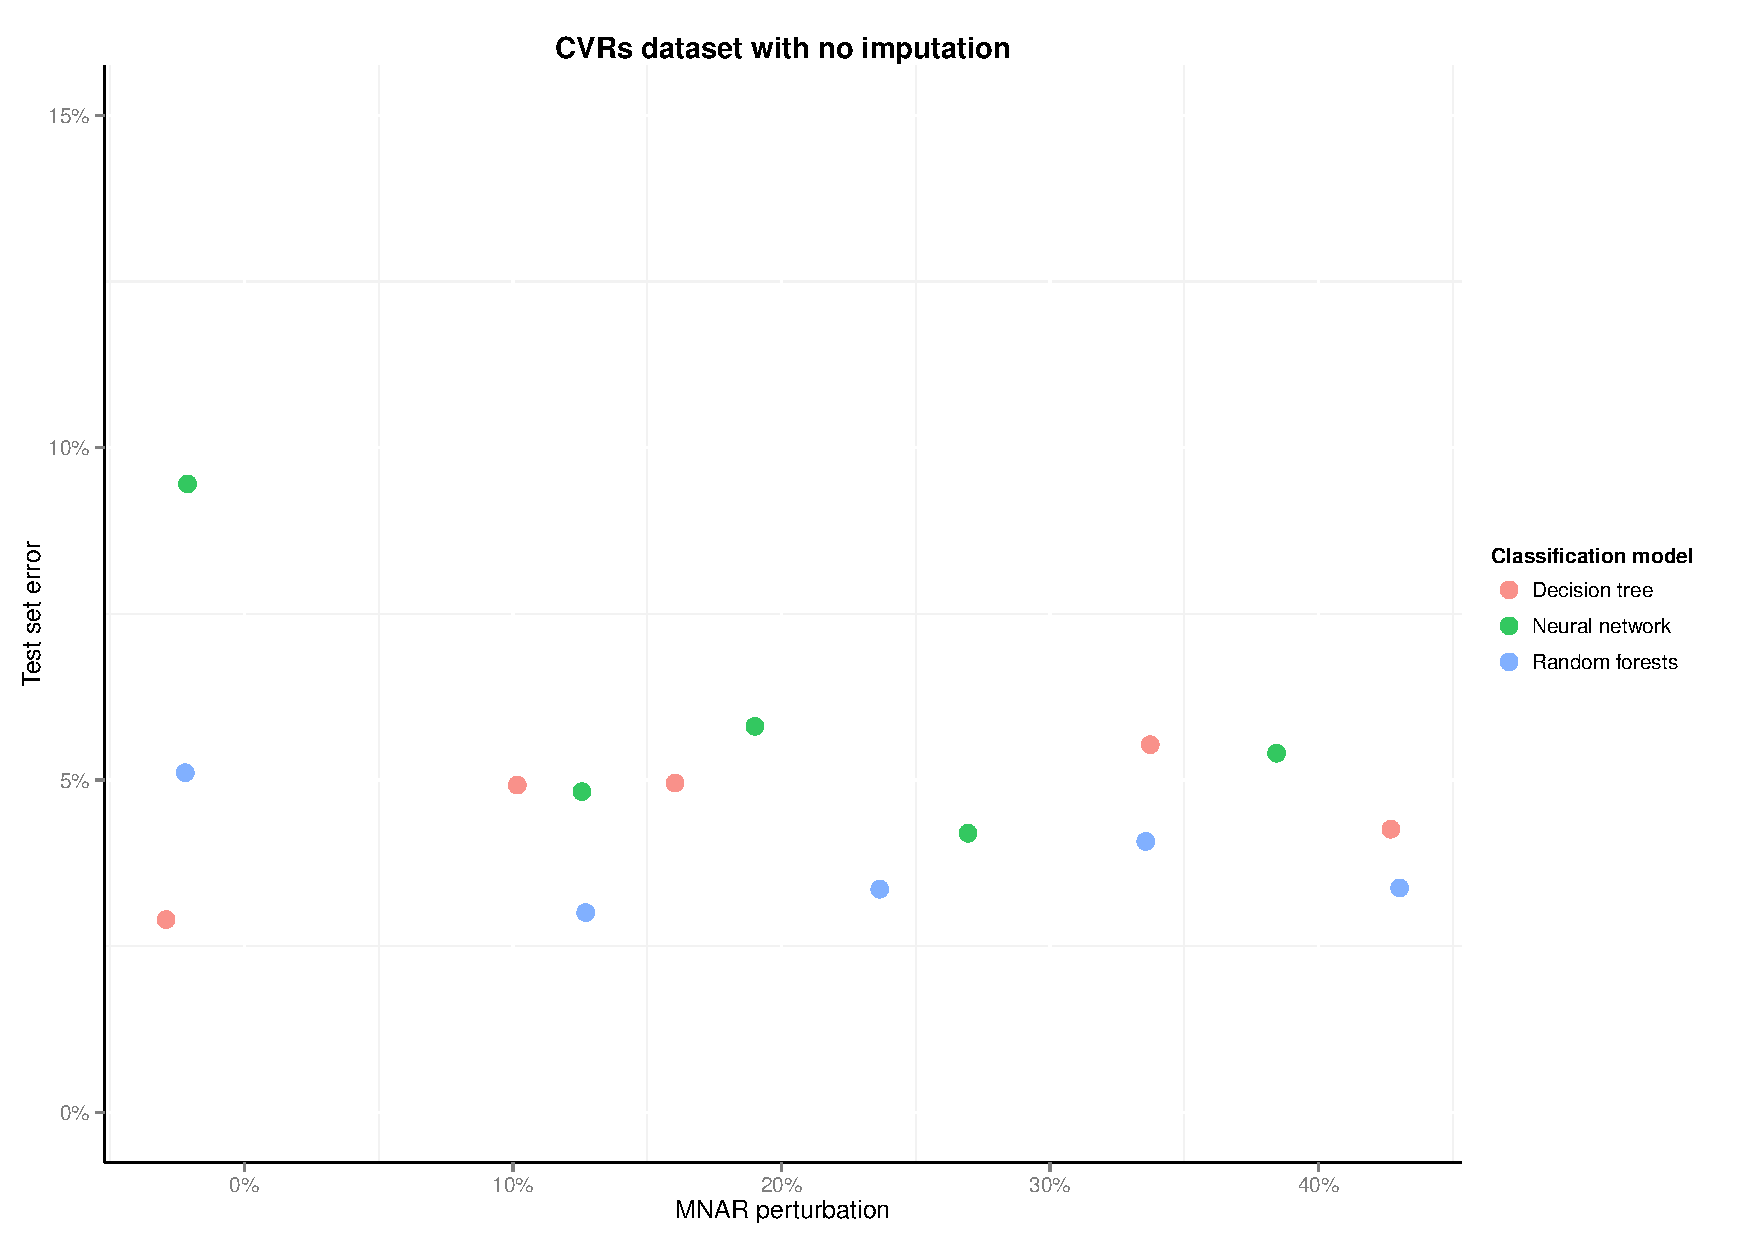
\includegraphics [scale=0.45]{figure/test-errors-votes-no-imp.pdf}\par
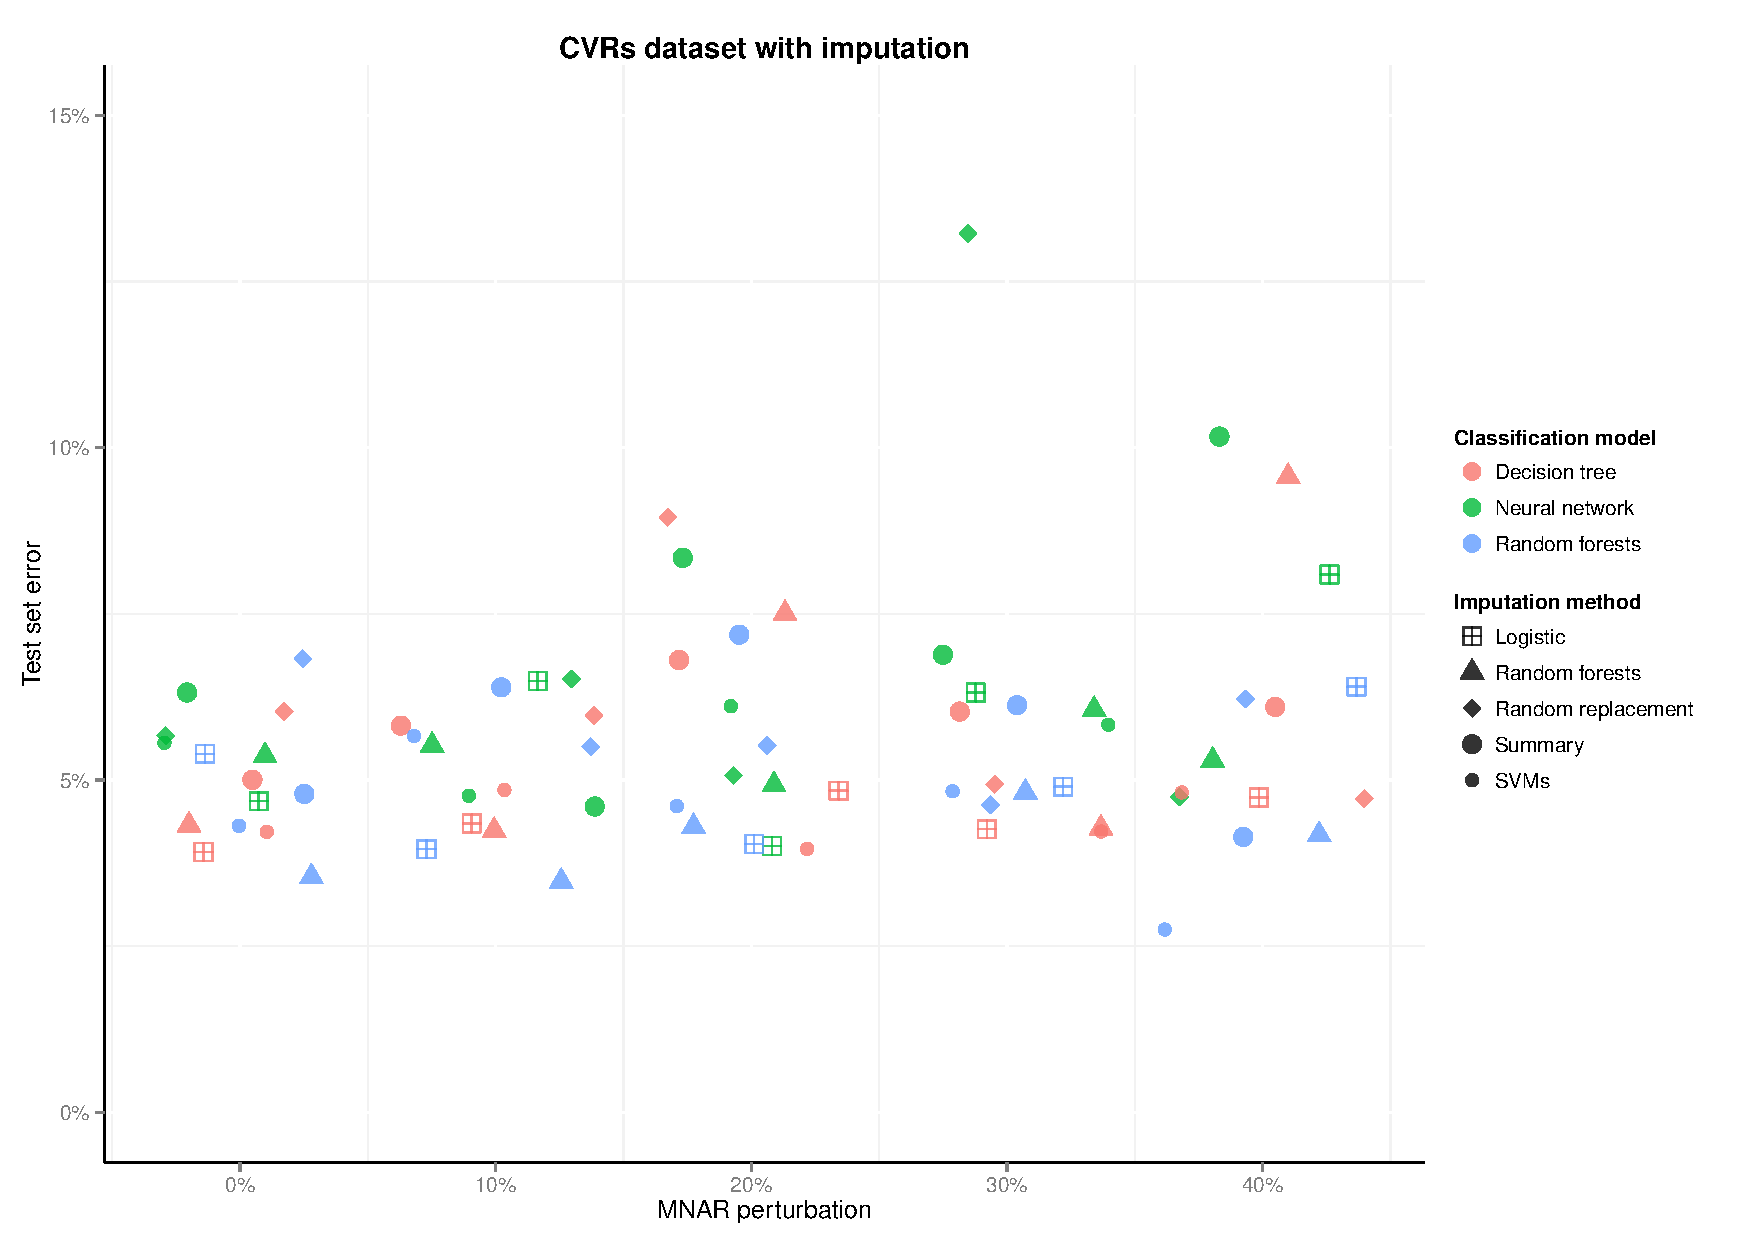
\includegraphics [scale=0.45]{figure/test-errors-votes-imp.pdf}\par
   \caption{\footnotesize Error rates on the CVRs test set with (bottom) and without (top) missing data imputation. See footnotes for Figure \ref{fig:test-error-adult}.}
   \label{fig:test-error-votes}
\end{figure}

\par

\setcounter{chapter}{4}
\setcounter{equation}{0} %-1
\noindent {\bf 4. Conclusion}  

Neural networks have become a popular machine learning algorithm in many domains, in part due to the ability of neural networks to ``learn'' how to engineer features.  However, researchers analyzing survey data typically choose decision trees or random forests for prediction tasks because missing data and categorical variables are not easy to handle with neural networks. This paper investigates techniques for handling missing data for training neural network classifiers. 

We compare the predictive performance of a four-layer neural network against decision tree and random forest classifiers trained on datasets with differently imputed data. We assess performance in terms of test set error for different levels of perturbed training data, from 0\% (no perturbation) to 40\% perturbation. We beat the state-of-the-art test error on the Adult dataset by 0.2\% using a random forests classifier trained on data imputed with logistic regression. Random forests trained on perturbed and one-hot encoded data outperforms the state-of-the-art on the CVRs dataset by over 2\%. 

We conclude from the results that the performance of the classifiers and imputation strategies generally depend on the nature and proportion of missing data. For the Adult dataset, random forests classifiers trained on data imputed with other classifiers outperform other classifiers and imputation methods across different ratios of perturbed data, while classifiers trained on one-hot encoded data perform very poorly on perturbed training data. This finding can be explained by the fact that missing values in the Adult dataset are concentrated in three features which may not be consequential for the prediction task, and perturbation exposes features that are more consequential to the prediction task to missing data. For the CVRs dataset, each of the three classifiers trained on one-hot encoded data perform well across different levels of perturbation. This finding can be explained by the fact that missing values represent potentially valuable information for the prediction task in the CVRs data.

For future work, we will further explore the idea that missing data may have more predictive value than imputed data in certain domains. A related question is whether neural networks can outperform decision trees or random forests trained on one-hot encoded data by learning different types of missing values. For instance, can neural networks engineer features that reflect the different types of missing values in the CVRs data, where missing values represent any action other than an up-or-down vote (e.g., voted present)? Answers to these questions will help guide researchers in choosing which imputation strategies and classifiers to use for prediction problems in different domains. 
\par
%%%%%%%%%%%%%%%%%%%%%%%%%%%%%%%%%%%%%%%%%%%%%%%%%%%%%%%%%%%%%%%%%%%%%%%%%%%%%%%%%%%%%%%%%%%%%%%%%%%%%%%%%%%%%%%%%%%%%%%%%%%%
\vskip 14pt
\noindent {\large\bf Supplementary Materials}

%Contain the brief description of the online supplementary materials.
The code used for this project is available on Github (\url{https://github.com/rafaelvalle/MDI}).

\par
%%%%%%%%%%%%%%%%%%%%%%%%%%%%%%%%%%%%%%%%%%%%%%%%%%%%%%%%%%%%%%%%%%%%%%%%%%%%%%%%%%%%%%%%%%%%%%%%%%%%%%%%%%%%%%%%%%%%%%%%%%%%
\vskip 14pt
\noindent {\large\bf Acknowledgements}

%Write the acknowledgements here.
We thank Isabelle Guyon for advice and the idea for the paper. We also thank Joan Bruna and seminar participants at the University of California, Berkeley for comments. This material is based upon work supported by the National Science Foundation Graduate Research Fellowship under Grant No. DGE 1106400. Any opinion, findings, and conclusions or recommendations expressed in this material are those of the authors and do not necessarily reflect the views of the National Science Foundation.
\par

%%%%%%%%%%%%%%%%%%%%%%%%%%%%%%%%%%%%%%%%%%%%%%%%%%%%%%%%%%%%%%%%%%%%%%%%%%%%%%%%%%%%%%%%%%%%%%%%%%%%%%%%%%%%%%%%%%%%%%%%%%%%
\markboth{\hfill{\footnotesize\rm JASON POULOS AND RAFAEL VALLE} \hfill}
{\hfill {\footnotesize\rm MISSING DATA IMPUTATION FOR NEURAL NETWORKS} \hfill}

\bibhang=1.7pc
\bibsep=2pt
\fontsize{9}{14pt plus.8pt minus .6pt}\selectfont
\renewcommand\bibname{\large \bf References} 
\clearpage
\markboth{\hfill{\footnotesize\rm JASON POULOS AND RAFAEL VALLE} \hfill}
{\hfill {\footnotesize\rm MISSING DATA IMPUTATION FOR NEURAL NETWORKS} \hfill}
%\begin{thebibliography}{11}
%\expandafter\ifx\csname
%natexlab\endcsname\relax\def\natexlab#1{#1}\fi
%\expandafter\ifx\csname url\endcsname\relax
%  \def\url#1{\texttt{#1}}\fi
%\expandafter\ifx\csname urlprefix\endcsname\relax\def\urlprefix{URL
%}\fi
%\bibitem[Antoine and Renault(2012)]{1} Antoine, B. and Renault, E. (2012). Efficient minimum distance
%estimation with multiple rates of convergence. \textit{J. Economet.} \textbf{170}, 350-367.
%\bibitem[Shao and Tu(1995)]{2}
%Shao, J. and Tu, D. (1995). \textit{The Jackknife and Bootstrap}. Springer-Verlag, New York.
%
%%%%%%%%%%%%%%%%%%%%%%%%%%%%%%%%%%%%%%%%%%%%%%%%%%%%%%%%%%%%%%%%%%%%%%%%%%%%%%%%%%%%%%%%%%%%%%%%%%%%%%%%%%%%%%%%%%%%%%%%%%%%%
%\end{thebibliography}
\bibliographystyle{apalike}
\bibliography{refs}

\vskip .65cm
\noindent
Department of Political Science, University of California, Berkeley, CA 94720-1950
\vskip 2pt
\noindent
E-mail: \href{mailto:poulos@berkeley.edu}{\nolinkurl{poulos@berkeley.edu}}
\vskip 2pt

\noindent
Center for New Music and Audio Technologies, University of California, Berkeley, CA 94720
\vskip 2pt
\noindent
E-mail: \href{mailto:rafaelvalle@berkeley.com}{\nolinkurl{rafaelvalle@berkeley.com}}
% \vskip .3cm
%\centerline{(Received ???? 20??; accepted ???? 20??)}\par
\end{document}
%%%%%%%%%%%%%%%%%%%%%%%%%%%%%%%%%%%%%%%%%%%%%%%%%%%%%%%%%%%%%%%%%%%%%%%%%%%%%%%%%%%%%%%%%%%%%%%%%%%%%%%%%%%%%%%%%%%%%%%%%%%%
%%%%%%%%%%%%%%%%%%%%%%%%%%%%%%%%%%%%%%%%%%%%%%%%%%%%%%%%%%%%%%%%%%%%%%%%%%%%%%%%%%%%%%%%%%%%%%%%%%%%%%%%%%%%%%%%%%%%%%%%%%%%

\end{document}
